\documentclass[11pt,a4paper]{article}
\usepackage[top=1.00in, bottom=1.0in, left=1.1in, right=1.1in]{geometry}
\usepackage{graphicx}
\usepackage{hyperref}
\usepackage[style=authoryear, backend=biber, natbib = true, style=numeric-comp, sortcites, hyperref, sorting=none, giveninits=true, doi=false,isbn=false,url=false,eprint=false, date=year, maxbibnames = 2, backend=bibtex]{biblatex}
\AtEveryBibitem{\clearfield{pages}}
\AtEveryBibitem{\clearlist{language}}
\AtEveryBibitem{%
  \clearfield{volume}%
  \clearfield{number}}
\AtEveryBibitem{\clearfield{title}}
\renewbibmacro{in:}{}
\usepackage[export]{adjustbox}
\usepackage[utf8x]{inputenc}
\usepackage{lmodern,textcomp}


\addbibresource{synchrony.bib} 

\begin{document}

\pagenumbering{gobble}

\noindent 
\includegraphics[width=0.5\textwidth, right]{../forestry_letterhead.png}

\vspace{0.5cm} 

\noindent Dear Editorial Office,
\vspace{0.35cm} 

\noindent I am writing to request a waiver of the article processing charges associated with the Brief Report entitled ``Solstice optimizes thermal growing season'' (2025-06796R).

\vspace{0.35cm}

\noindent This research was conducted during a short-term visit I undertook in August 2024 while I was still a PhD student. My visit was supported by a small travel grant intended to facilitate international collaboration for young researchers (grant \href{https://www.umontpellier.fr/en/articles/appel-a-projets-explore6-soutien-aux-mobilites-internationales}{EXPLORE6}, funded by University of Montpellier). While the grant covered travel and living expenses (for a total amount of €5,196.16---see letter of grant acceptance attached, in French), it did not include any support for publication costs. 

\vspace{0.35cm}

\noindent The project was not attached to any larger grant, and my PhD fellowship only covered my salary as a PhD student for three years. The host university (University of British Columbia) that welcomed me during my stay also does not have dedicated funding to support publication fees. 

\vspace{0.35cm}

\noindent Given these circumstances, I am currently unable to cover the APC. I would be sincerely grateful if the journal could consider a waiver of the publication fees, so that the results of this project may be made accessible to the research community.

\vspace{0.35cm}

\noindent Please do not hesitate to contact me if you need any additional information to support this request. I sincerely thank you for your consideration and understanding.

\vspace{0.45cm}
\noindent Sincerely, 
\vspace{0.45cm}\\
\hspace*{-0.5cm}
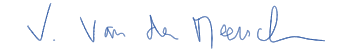
\includegraphics[scale=.65]{../sign_long.png} \\
\noindent Victor Van der Meersch, PhD\\
\noindent \emph{Forest \& Conservation Sciences}\\
\noindent \emph{University of British Columbia}

\newpage

\end{document}








